\chapter{Programm}
\label{chap:Programm}

\section{Parameter des Fluggeräts}
\label{sec:parameter_fluggeraet}
Bei der Auslegung des Fluggeräts werden nicht nur Multicopter betrachtet sondern auch Flächenflugzeuge, sogenannte fixed wing UAVs. Aus diesem Grund werden die Parameter Motor, Propeller, Batterie und Missionsparameter sowie Umgebungsparameter allgemein für beide Arten der UAVs festgelegt. Anschließend werden die Parameter des Multicopters oder des Flächenflugzeugs festgelegt, je nachdem, welches Fluggerät untersucht werden soll. 
Das Programm und die diesem grundlegende Leistungsberechnung, basieren auf der unveröffentlichten Arbeit "Leistungsberechnung von Multicoptern" von Y. Beyer (2016). Aus dieser wurden die Berechnung der Aerodynamik von Multicoptern, die Pulsweitenmodulation und der Batterieentladung übernommen. 
 
\subsubsection{Flugsystem}
Zu Beginn der Mission muss das Flugsystem festgelegt werden, da jeweils nur eins zu jedem Zeitpunkt untersucht werden kann. Die Abfrage erfolgt mit der Variablen \texttt{Abfrage\_Flugsystem}. Diese kann die Werte 1 für einen Multicopter oder 0 für ein Flächenflugzeug annehmen.

\subsubsection{Motor}
Die ersten drei Motorparameter sind notwendig, um die Motorspannung und den Motorstrom zu berechnen. Der letzte Parameter dint als technische Grenze, die für ein gut ausgelegtes System nicht überschritten wird. Die Motormasse fließt in Kombination mit der Anzahl der Propeller in die Gesamtmasse des Fluggerätes mit ein.

\begin{center}
	\captionof{table}{Motorparameter für technische Grenzen}
	\begin{tabular}{l l l} \hline
		 Parameter & Variablenname & Einheit \\ \hline
		 Innenwiderstand \ensuremath{R_i} & \texttt{R\_i} & \SI{}{\ohm} \\
		 Geschwindigkeitskonstante \ensuremath{K_v} & \texttt{K\_V} & \ensuremath{\frac{RPM}{V}} bzw. \ensuremath{\frac{U}{Vs}} \\
		 Leerlaufstrom \ensuremath{I_0} & \texttt{I\_O} & \ensuremath{A}  \\
		 maximaler Dauerstrom \ensuremath{I_{max}} & \texttt{I\_max} & \ensuremath{A} \\
		 Motormasse \ensuremath{m_{Mot}} & \texttt{m\_Mot} & \ensuremath{kg} \\ \hline
	\end{tabular}	
	\label{tab:mot_parameter}
\end{center}

\subsubsection{Propeller}
Der Propellername wird in der Form 'Durchmesser x Pitch' angegeben. Der Name ist wichtig, um das Propellerkennfeld aus Propellerdatenbank von APC zu entnehmen. Die Anzahl der Propeller beeinflusst entscheidend die Geometrie des Fluggerätes. Weiterhin wird damit der benötigte Schub auf die Anzahl der Propeller aufgeteilt. Die letzten Parameter dienen zur Bestimmung Anströmung und der Berücksichtigung der Blattelemententheorie.


\begin{center}
	\captionof{table}{Propellerparameter für Schub, aerodynamische und technische Grenzen}
	\begin{tabular}{l l l} \hline
		 Parameter & Variablenname & Einheit \\ \hline
		 Propellername & \texttt{prop\_name} & \ensuremath{-} \\
		 Anzahl der Propeller \ensuremath{n_{Prop}} & \texttt{n\_Prop} & \ensuremath{-} \\
		 Mittlerer Nullwiderstandsbeiwert \ensuremath{c_{d0}} & \texttt{c\_d0} & \ensuremath{0,05} \\
		 Anstieg des Auftriebsbeiwerts \ensuremath{\frac{dc_a}{dc_\alpha}} & \texttt{a\_alpha} & \ensuremath{5} \\
		 Maximaler Anstellwinkel \ensuremath{\alpha_{max}} & \texttt{alpha\_stall} & \ensuremath{10}\textdegree \\ \hline
	\end{tabular}	
	\label{tab:prop_parameter}
\end{center}

\subsubsection{Batterie}
Die aufgeführten Parameter der Batterie bestimmen zum einen die verfügbare Kapazität und zum anderen die Batterieentladung. Bei der Energiedichte handelt es sich um repräsentative Werte für den verwendeten Akkutyp, z.B. Li-Ion oder Li-Po. Die minimale Zellenspannung ist ein Erfahrungswert, der am \textit{Institut für Flugführung} verwendet wird. Um den Energieverlust der Batterie zu berechnen, wird die Peukert konstante herangezogen. Diese beträgt für Li-Po-Akkus ca. $1,01 \leq P \leq 1,05$ und für Li-Ion-Akkus ca. 1,05 (Traub). Außerdem sind Lithium Batterien stark temperaturempfindlich. Niedrige Temperaturen als die Umgebungstemperatur können die angegebene Nennkapazität reduzieren und die Verluste progressiv steigen lassen. Die maximale C-Rate dient als weitere technische Begrenzung, die wiederum für ein gut ausgelegtes System nicht erreicht wird.


\begin{center}
	\captionof{table}{Batterieparameter zur Berechnung der verbleibenden Restladung sowie der technischen Grenzen}
	\begin{tabular}{l l l} \hline
		 Parameter & Variablenname & Einheit \\ \hline
		 Energiedichte \ensuremath{\frac{E_{Bat}}{m_{Bat}}}& \texttt{E\_Dichte} & \ensuremath{J/kg} \\
		 Anzahl der Batteriezellen \ensuremath{N_{Bat,cell}} & \texttt{N\_bat\_cell} & \ensuremath{-} \\
		 nominale Spannung pro Batteriezelle \ensuremath{U_{Bat,cell}} & \texttt{U\_bat\_nom} & \ensuremath{V} \\
		 minimale Spannung pro Batteriezelle \ensuremath{U_{Bat,cell,min}} & \texttt{U\_bat\_min} & \ensuremath{V} \\
		 Peukert-Konstante \ensuremath{P}& \texttt{P\_bat\_Peukert} & \ensuremath{1,05} \\
		 Maximale C-Rate \ensuremath{C_{rate,max}} & \texttt{C\_Rate\_max} & \ensuremath{-} \\
		 Batteriemasse \ensuremath{m_{Bat}} & \texttt{m\_bat} & \ensuremath{kg} \\ \hline
	\end{tabular}	
	\label{tab:bat_parameter}
\end{center}

\subsubsection{Multicopter}
Die Parameter für den Multicopter sind in \ref{tab:multicop_parameter} aufgeführt. Die Leermasse fließt mit in die Gesamtmasse mit ein und wird für die Berechnung des Schubs und weiterer Parameter benötigt. Die Beiwerte sind reine Schätzwerte. Für die nachfolgenden Berechnungen ist nur die obere Stirnfläche von Bedeutung, da sich auf diese die Beiwerte beziehen. Die Propeller bleiben bei den Stirnflächen unberücksichtigt.
\begin{center}
	\captionof{table}{Parameter des Multicopters}
	\begin{tabular}{l l l} \hline
		 Parameter & Variablenname & Einheit \\ \hline
		 Leermasse des Multicopters \ensuremath{m_{Copter}} & \texttt{m\_copter} & \ensuremath{kg}\\
		 Obere Stirnfläche \ensuremath{A_{copter,oben}} & \texttt{A\_copter} & \ensuremath{m^2}\\
		 seitliche Stirnfläche \ensuremath{A_{copter,seitlich}} & \texttt{A\_copter\_seitlich} & \ensuremath{m^2}\\
		 Oberer Widerstandsbeiwert \ensuremath{c_{W,copter,oben}} & \texttt{c\_W\_copter\_oben} & \ensuremath{-}\\
		 Seitlicher Widerstandsbeiwert \ensuremath{c_{W,copter,seitlich}} & \texttt{c\_W\_copter\_seitlich} & \ensuremath{-}\\
		 Maximaler Auftriebsbeiwert \ensuremath{c_{A,copter,max}} & \texttt{c\_A\_copter\_max} & \ensuremath{-}\\ \hline
	\end{tabular}	
	\label{tab:multicop_parameter}
\end{center}

\subsubsection{Flächenflugzeug}
Der erste Parameter des Flächenflugzeugs wird zur Ermittlung des Bahnanstellwinkels benötigt. Für den Steigflug wird ein Flug mit optimaler Gleitzahl \ensuremath{E} vorausgesetzt. Mit der Leermasse wird analog zum Multicopter der Schub berechnet.
\begin{center}
	\captionof{table}{Parameter des Flächenflugzeug}
	\begin{tabular}{l l l} \hline
		 Parameter & Variablenname & Einheit \\ \hline
		 Reziproke Gleitzahl \ensuremath{\varepsilon} & \texttt{epsilon} & \ensuremath{-}\\		 
		 Leermasse des Flächenflugzeug \ensuremath{m_{Flugzeug}}& \texttt{m\_flugzeug} & \ensuremath{kg}\\ \hline
	\end{tabular}	
	\label{tab:flugzeug_parameter}
\end{center}

\section{Parameter der Mission}
\label{sec:parameter_mission}

\subsubsection{Flugparameter}

\subsubsection{Umgebungsparameter}
Die Erdbeschleunigung und der Adiabatenexponent werden als konstant über der Höhe angenommen. Mit Startwerten für die Höhe, die Temperatur, die Dichte und des Luftdrucks werden die Abflugbedingungen am Abflugort spezifiziert. Mit der Schrittweite der Höhe wird die Genauigkeit der Höhendiskretisierung festgelegt.
\begin{center}
	\captionof{table}{Umgebungsparameter}
	\begin{tabular}{l l l} \hline
		 Parameter & Variablenname & Einheit \\ \hline
		 Erdbeschleunigung \ensuremath{g} & \texttt{g} & 9,81 \ensuremath{m/s^2} \\
		 Starthöhe \ensuremath{H_0} & \texttt{H\_0} & \ensuremath{m} \\
		 Schrittweite der Höhe  \ensuremath{\Delta H} & \texttt{Delta\_H} & \ensuremath{m} \\
		 maximale Höhe \ensuremath{H_{max}} & \texttt{H\_max} & \ensuremath{m} \\
		 Umgebungstemperatur am Start \ensuremath{T_0} & \texttt{T\_0} & \ensuremath{K} \\
		 Luftdruck am Start \ensuremath{p_0} & \texttt{p\_0} & \ensuremath{N/m^2} \\
		 Dichte am Start \ensuremath{\rho_0} & \texttt{rho\_0} & \ensuremath{N/m^3} \\
		 Adiabatenexponent \ensuremath{\kappa} & \texttt{kappa} & \SI{1,4}{} \\
		 Windgeschwindigkeit \ensuremath{u_{Wg}} & \texttt{u\_Wg} & \ensuremath{m/s} \\ \hline
	\end{tabular}	
	\label{tab:prop_parameter}
\end{center}

\section{Berechnung weiterer Parameter}

\section{Parameter der Mission}

\section{Aufbau des Programms}
\label{sec:aufbau_des_programms}
Der Aufbau des \textsc{Matlab}-Skriptes wird im Struktogramm (abb. blabla) verdeutlicht.
%\begin{figure}[H]
%\centering
%	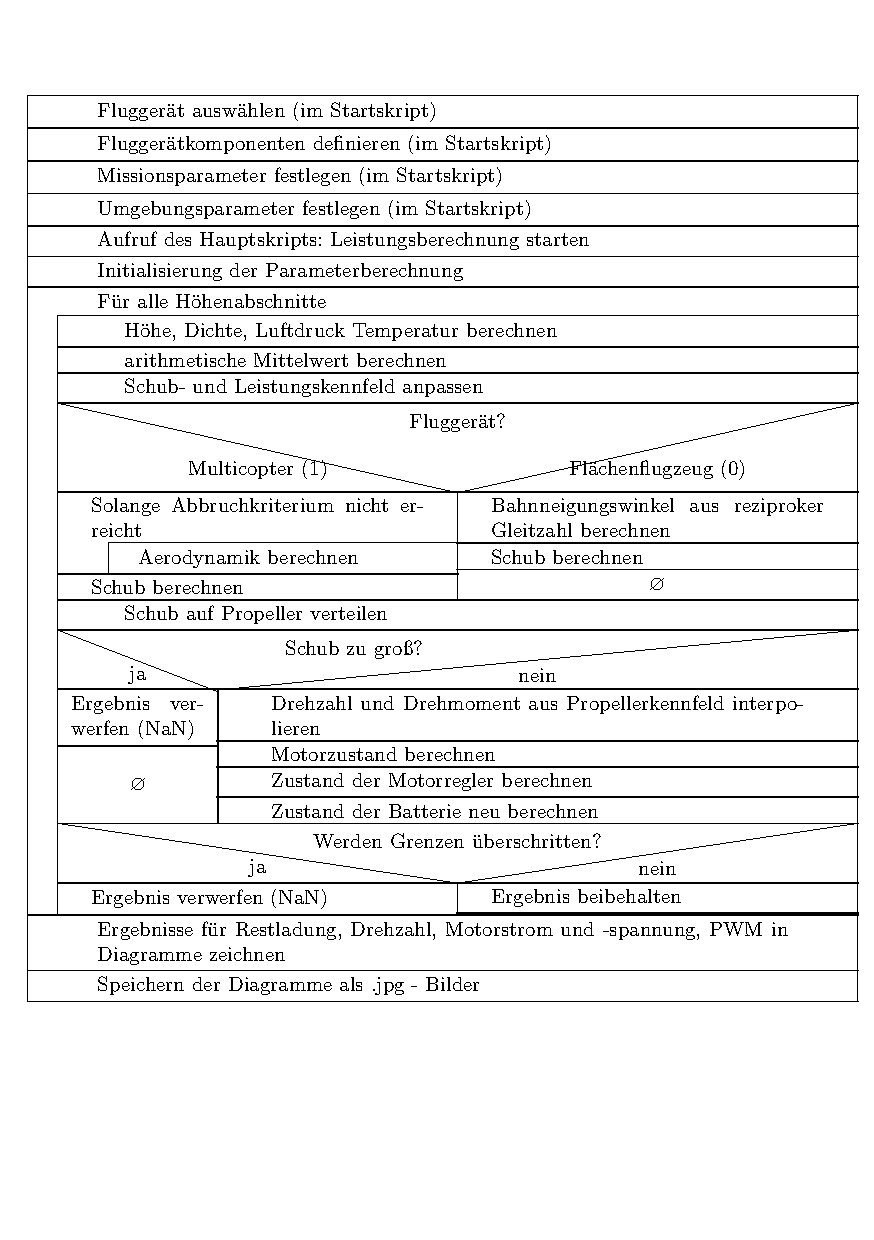
\includegraphics{Struktogramm.pdf}
%	\caption{Struktogramm des MATLAB-Skripts}
%	\label{abb:struktogramm}
%\end{figure}
\section{Leistungsberechnung}
\label{sec:leistungsberechnung}
\subsection{Veränderung der Umgebungsparameter mit der Höhe}
Für Leistungsuntersuchung wird die Internationale Standardatmosphäre vorausgesetzt. Hiernach ist der Temperaturkoeffizient bis zur Tropopause
\begin{equation}
	\frac{dT}{dH} = -0,0065\frac{K}{m}
\end{equation}
und danach in der unteren Stratosphäre bis zu einer Höhe von \SI{20000}{m}
\begin{equation}
	\frac{dT}{dH} = 0.
\end{equation}
Entsprechend kann der Verlauf der Temperatur, des Druckes und der Dichte mit
\begin{equation}
	T_{0-11} = T_0 - \frac{dT}{dH}\cdot H,
\end{equation}
\begin{equation}
	p_{0-11} = p_0\cdot [1-0,0065\frac{K}{m}\cdot \frac{H}{T_0}]^{5,256},
\end{equation}
\begin{equation}
	\rho_{0-11} = \rho_0 \cdot [1-\frac{dT}{dH}\cdot \frac{H}{T_0}]^{4,256}
\end{equation}
beschrieben werden. Ab \SI{20000}{m} ist der Verlauf von Druck und Dichte durch die Gleichungen
\begin{equation}
	p = p_{11}\cdot e^{\frac{g}{R\cdot T_{11}}\cdot (H-H_{11})},
\end{equation} 
\begin{equation}
	\rho = \rho_{11}\cdot e^{\frac{g}{R\cdot T_{11}}\cdot (H-H_{11})}
\end{equation}
gegeben.
Um den Einfluss der Flughöhe in der Leistungsberechnung festzuhalten, werden für jedes Höhenintervall die Umgebungsparameter an den oberen und unteren Intervallgrenzen berechnet. Daraus ergibt sich  

\subsection{Schub berechnen}
\subsubsection{Multicopter}
\subsubsection{Flächenflugzeug}
\subsection{Drehzahl und Drehmoment aus Propellerkennfeld interpolieren}
In der Propellerdatenbank von Hersteller APC sind zu jedem Propeller dieser Marke die Kennfelder aus Standschubversuchen aufgeführt. Die Art der Aufführung lässt allerdings keine Interpolation der Drehzahl bzw. des Drehmomentes in Abhängigkeit des Schubes und der absoluten Fluggeschwindigkeit zu. Aus diesem Grund muss das Kennfeld auf uniforme Geschwindigkeitsabstände transformiert werden. Dazu wird ein Geschwindigkeitsvektor mit Abständen von \SI{1}{m/s} gebildet. Die Funktion \texttt{Propeller\_map} (entommen aus Beyer, Y. (2016)) interpoliert danach das Schub- und Leistungskennfeld neu über der Geschwindigkeit und Drehzahl. Mit dem zuvor berechneten Schub und der absoluten Fluggeschwindikeit kann schließlich mit der Funktion \texttt{Propeller} die Drehzahl und das Drehmoment mittels linearer Interpolation ermittelt werden.
Die Kennfelder wurden in Versuchen ermittelt, die keine ändernde Dichte berücksichtigen. Um den Einfluss der sich verringernden Dicht mit zunehmender Flughöhe trotzdem zu beachten, müssen die Kennfelder angepasst werden. Gemäß der Strahltheorie setzt sich der Schub aus dem Massenstrom und der Geschwindigkeit im voll ausgebildeten Abstromzylinder 
\begin{equation}
	T =  \dot{m}\cdot v_{\infty} = \rho\cdot A_{Propeller}\cdot v_i\cdot v_{\infty}
\end{equation}
zusammen. Unter der Annahme gleicher induzierter Geschwindigkeiten $v_i$ und gleicher Geschwindigkeiten im voll ausgebildeten Abstrom $v_{\infty}$
\begin{equation}
	\frac{T_1}{T_2} = \frac{\rho_1}{\rho_2}
\end{equation}
kann das Schubfeld des Propellers an den Höheneinfluss angepasst werden.

\subsection{Motorzustand berechnen}
Mit dem Drehmoment und der Drehzahl des Propellers berechnet sich der Motorzustand, genauer der Motorstrom und die Motorspannung. Dies erfolgt nach einem einfachen Motormodell (Drela 2007).
Der Motorstrom berechnet sich aus 
\begin{equation}
	I_{Mot} = Q\cdot K_v + I_0.
\end{equation}
Mit dem Strom ergibt sich die Spannung nach
\begin{equation}
	U_{Mot} = \frac{\omega}{K_v} + R_i\cdot I_{Mot}.
\end{equation}
\subsection{Zustand der Motorregler}

\begin{equation}
\eta_{ESC} = \begin{cases} 
0,7\cdot PWM + 0,50 & wenn 0 < PWM \leq 0,5 \\ 
0,2\cdot PWM + 0,75 & wenn 0,5 < PWM \leq 1 \\ 
undefiniert & sonst 
\end{cases}
\end{equation}
wobei die Pulsweitenmodulation 
\begin{equation}
	PWM = \frac{U_{mot}}{U_{Bat}}
\end{equation}
mit dem Spannungsverhältnis des ESCs berechnet wird.
\subsection{Batteriezustand}
Die wesentliche Zustandsgröße der Batterie ist der Entladestrom \ensuremath{I_{Bat}}. Dieser setzt sich aus den einzelnen Motorströmen zusammen und zusätzlich dem Wirkungsgrad der Pulsweitenmodulation
\begin{equation}
	I_{Bat} = I_{Mot}\cdot \frac{PWM}{\eta_{PWM}}\cdot n_{Prop}.
\end{equation}


\subsection{Werden Grenzen überschritten?}
\section{Einschränkungen und Annahmen}